\documentclass{article}

% ================================================================
% Idioma y codificación
% ================================================================
\usepackage[spanish]{babel}
\usepackage[T1]{fontenc}
\usepackage[utf8]{inputenc}

% ================================================================
% Gráficos y layout
% ================================================================
\usepackage{graphicx}
\graphicspath{{imagenes/}}
\usepackage[colorlinks=true, allcolors=blue]{hyperref}
\usepackage[letterpaper,top=2cm,bottom=5cm,left=3cm,right=3cm,marginparwidth=1.75cm]{geometry}

% ================================================================
% Matemáticas y símbolos
% ================================================================
\usepackage{amsmath}
\usepackage{amssymb}

% ================================================================
% Tablas y color
% ================================================================
\usepackage{tabularx}
\usepackage{array}
\usepackage{colortbl}
\usepackage{xcolor}
\definecolor{headerblue}{RGB}{30,60,120}

% ================================================================
% Listas, figuras y formato
% ================================================================
\usepackage{enumitem}
\usepackage{float}
\usepackage{subcaption}
\usepackage{fancyhdr}
\usepackage{parskip}

\pagestyle{fancy}
\fancyhf{}
\setlength{\headheight}{70pt}

% Definición del encabezado
\fancyhead[C]{%
    \begin{minipage}[c]{1.5cm}
        \includegraphics[width=1.5cm]{imagenes/uta.png}
    \end{minipage}%
    \hfill
    \begin{minipage}[c]{10cm}
        \centering
        \small {\textbf{UNIVERSIDAD TÉCNICA DE AMBATO}} \\[0.1cm]
        \scriptsize \textit{FACULTAD DE INGENIERÍA EN SISTEMAS ELECTRÓNICA E INDUSTRIAL} \\[0.1cm]
        \scriptsize \textbf{CARRERA SOFTWARE} \\[0.1cm]
        \scriptsize \textbf{CICLO ACADÉMICO: JULIO - DICIEMBRE 2026}
        \vspace{0.2cm}
    \end{minipage}%
    \hfill
    \begin{minipage}[c]{1.5cm}
        \centering
        \includegraphics[width=1.5cm]{imagenes/fisei.png}
    \end{minipage}%
}
\fancyfoot[C]{\thepage}

\begin{document}
\begin{center}
    {\large \textbf{INFORME DE GUÍA PRÁCTICA}} \\
\end{center}

% ================================================================
\section{Portada}
% ================================================================
\begin{flushleft}
\begin{tabular}{ l p{9cm} }
    \textbf{Tema:} & APE 6. Evaluación y validación — Fase 2: Pilotaje \\
    \textbf{Unidad de Organización Curricular:} & Profesional \\
    \textbf{Nivel y Paralelo:} & 5 - A \\
    \textbf{Alumnos participante(s):} & Cholota Bastidas Ariel Isai \\
                                      & García Amores Manolo José \\
                                      & Miranda Tarupi Luis Sebastián \\
                                      & Velasco Huayamave Kevin Andrés \\
    \textbf{Asignatura:} & Interacción Humano/Computador \\
    \textbf{Docente:} & Ing. Caiza Caizabuano Jose Ruben \\
\end{tabular}
\end{flushleft}

% ================================================================
\section{Informe de guía práctica}
% ================================================================

\subsection{Objetivos}
\subsubsection{General}
Ejecutar el pilotaje del protocolo de evaluación de usabilidad del prototipo \textbf{CaféU} con tres participantes reales del perfil, calcular las métricas de eficacia, eficiencia y satisfacción (ISO 9241-11), aplicar la evaluación heurística individual y documentar los ajustes del protocolo (versión 1 $\rightarrow$ versión 2), identificando problemas de interacción que sirvan de base para las Fases 3 y 4.

\subsubsection{Específicos}
\begin{itemize}[leftmargin=1.5em, itemsep=2pt]
    \item Verificar que el repositorio GitHub contenga los artefactos de la Fase 1 (plan de evaluación, consentimiento informado, seis tareas, métricas, cuestionario SUS y hoja de observación).
    \item Ejecutar las seis tareas planificadas con al menos tres participantes del perfil, aplicando el consentimiento informado y la técnica de pensamiento en voz alta.
    \item Registrar los tiempos, el éxito, los errores críticos/no críticos y las dificultades observadas.
    \item Calcular la tasa de éxito por tarea, la mediana del tiempo, los errores y el puntaje SUS por participante.
    \item Documentar los ajustes del protocolo (versión 1 $\rightarrow$ versión 2) a partir de los criterios de validación de la Fase 1.
    \item Realizar la evaluación heurística individual (10 heurísticas de Nielsen) y compararla con los resultados del pilotaje.
    \item Listar los hallazgos preliminares para las Fases 3 y 4.
\end{itemize}

\subsection{Modalidad}
Presencial

\subsection{Tiempo de duración}
Presenciales: 3\\
No presenciales: 1

\subsection{Instrucciones}
\textbf{Acciones previas:}
\begin{itemize}[leftmargin=1.5em, itemsep=2pt]
    \item Revisar que el repositorio GitHub contenga los artefactos de la Fase 1.
    \item Seleccionar tres participantes que cumplan el perfil (estudiantes UTA, ajenos al diseño del prototipo, mayores de edad).
    \item Tener el prototipo CaféU abierto y en su estado inicial, con internet probado.
    \item Preparar un solo cronómetro, una hoja de observación por participante y el guion de consentimiento, las tareas y la pista escrita a la mano del moderador.
    \item Realizar un ensayo interno: un integrante ejecuta todas las tareas (no cuenta como dato) y se prueba el reinicio del prototipo.
\end{itemize}

\textbf{Pasos:}
\begin{enumerate}[leftmargin=1.5em, itemsep=2pt]
    \item Aplicar el consentimiento informado y verificar el perfil del participante.
    \item Ejecutar las seis tareas cronometradas aplicando el pensamiento en voz alta.
    \item Registrar tiempos, éxito, errores y dificultades en la hoja de observación.
    \item Aplicar el cuestionario SUS al finalizar cada sesión.
    \item Reiniciar el prototipo entre participantes y comprobar el estado inicial.
    \item Transcribir los datos por participante (P1, P2 y P3) sin modificar ni inventar.
    \item Calcular las métricas, revisar los criterios del protocolo y registrar los ajustes (V1 $\rightarrow$ V2).
    \item Realizar la evaluación heurística individual y compararla con el pilotaje.
    \item Listar los hallazgos preliminares y elaborar el informe final.
\end{enumerate}

\subsection{Listado de equipos, materiales y recursos}
\textbf{Listado de equipos y materiales generales empleados en la guía práctica:}
\begin{itemize}[leftmargin=1.5em, itemsep=3pt]
    \item Computadora
    \item Herramientas ofimáticas
    \item Aula virtual
    \item Internet
    \item Visual Studio Code
    \item Navegador web (Chrome) y cronómetro
    \item Prototipo CaféU (HTML, CSS y JavaScript)
    \item Hojas de observación impresas y guion de consentimiento
\end{itemize}

\textbf{TAC (Tecnologías para el Aprendizaje y Conocimiento) empleados en la guía práctica:}
\begin{itemize}[leftmargin=1.5em, itemsep=2pt]
    \item[$\square$] Plataformas educativas
    \item[$\square$] Simuladores y laboratorios virtuales
    \item[$\square$] Aplicaciones educativas
    \item[$\square$] Recursos audiovisuales
    \item[$\square$] Gamificación
    \item[$\blacksquare$] Inteligencia Artificial
    \item Otros (Especifique): \underline{\hspace{5cm}}
\end{itemize}

\subsection{Actividades por desarrollar}
\begin{enumerate}[leftmargin=1.5em, itemsep=2pt]
    \item \textbf{Verificación de la Fase 1:} revisar que el repositorio contenga el plan de evaluación, el consentimiento informado, las seis tareas, las métricas, el cuestionario SUS y la hoja de observación. \textbf{Producto:} carpeta \texttt{ape6/Fase1/}.
    \item \textbf{Ejecución del pilotaje:} aplicar el consentimiento, ejecutar las seis tareas con tres participantes y registrar los datos con pensamiento en voz alta. \textbf{Producto:} hojas llenas y anonimizadas.
    \item \textbf{Registro de resultados:} crear un archivo individual por participante (P1, P2 y P3) sin modificar ni inventar los datos. \textbf{Producto:} \texttt{Fase2-Pilotaje/Participantes/}.
    \item \textbf{Cálculo de métricas:} tasa de éxito, mediana del tiempo, errores críticos/no críticos y puntaje SUS. \textbf{Producto:} resumen de métricas.
    \item \textbf{Ajustes del protocolo:} comparar los resultados con los criterios de la Fase 1 y documentar la tabla V1 $\rightarrow$ V2. \textbf{Producto:} ajustes del protocolo.
    \item \textbf{Evaluación heurística individual:} cada integrante evalúa el prototipo con las 10 heurísticas de Nielsen y se compara con el pilotaje. \textbf{Producto:} evaluaciones heurísticas.
    \item \textbf{Hallazgos preliminares:} documentar los problemas, la tarea afectada, los participantes involucrados, la evidencia y la heurística incumplida. \textbf{Producto:} hallazgos para las Fases 3 y 4.
\end{enumerate}

\subsection{Resultados obtenidos}

\subsubsection{Protocolo de evaluación (resumen de la Fase 1)}
En la Fase 1 se planificó la evaluación de usabilidad del prototipo \textbf{CaféU}, una aplicación web móvil que permite a los estudiantes universitarios pedir en la cafetería antes de llegar.

\begin{itemize}[leftmargin=1.5em, itemsep=2pt]
    \item \textbf{Pregunta de evaluación (ISO 9241-11):} ¿en qué medida el prototipo CaféU permite consultar el menú y realizar pedidos con eficacia, eficiencia y satisfacción, y qué problemas de usabilidad lo impiden?
    \item \textbf{Métodos (triangulación):} evaluación heurística (analítico, 10 heurísticas de Nielsen) y prueba con usuarios con pensamiento en voz alta (empírico).
    \item \textbf{Perfil de participantes:} 3 estudiantes universitarios de la UTA, ajenos al diseño del prototipo, mayores de edad. Se identifican con los códigos P1, P2 y P3.
    \item \textbf{Métricas:} tasa de éxito (eficacia), mediana del tiempo (eficiencia), errores críticos/no críticos (eficacia y eficiencia) y SUS (satisfacción).
    \item \textbf{Roles:} moderador (Luis Miranda), registro de métricas (Kevin Velasco), observador (Manolo García) y soporte técnico (Ariel Cholota).
\end{itemize}

\subsubsection{Prototipo funcional CaféU}
Se completó el prototipo CaféU como una aplicación funcional de una sola página con cinco pantallas (Inicio, Menú, Detalle, Mi pedido y Confirmación), un catálogo de seis productos (tres bebidas y tres comidas), filtros por categoría, buscador, selector de cantidad, modificación/eliminación de ítems, cálculo del subtotal y generación del código de retiro \texttt{\#CU-104}. El pedido se mantiene solo en memoria, por lo que recargar la página restablece el estado inicial entre participantes.

\begin{figure}[H]
    \centering
    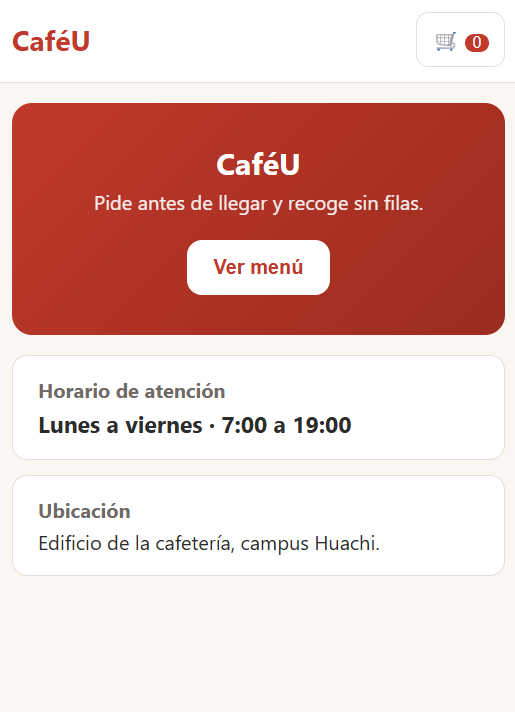
\includegraphics[width=0.48\textwidth]{imagenes/pantalla-inicio.png}
    \hfill
    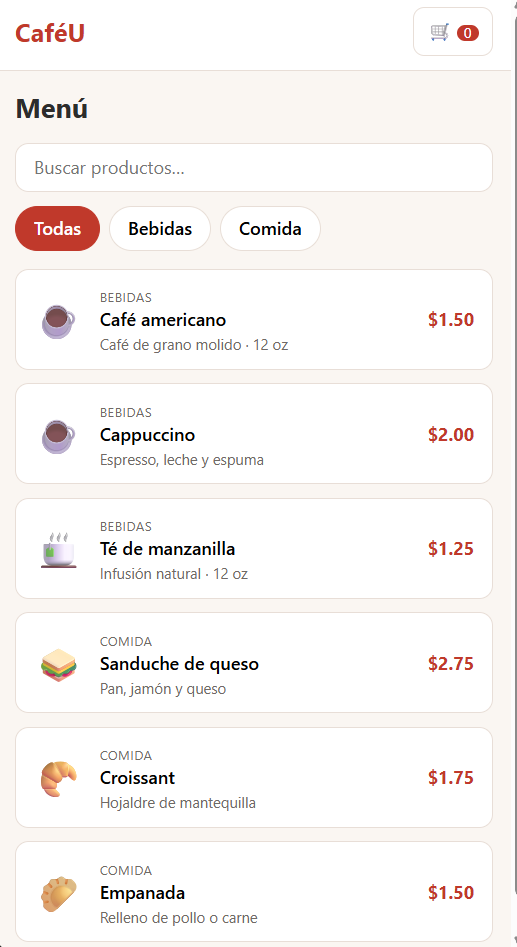
\includegraphics[width=0.48\textwidth]{imagenes/pantalla-menu.png}
    \caption{Pantallas Inicio (horario de atención) y Menú (catálogo con filtros).}
    \label{fig:inicio-menu}
\end{figure}

\begin{figure}[H]
    \centering
    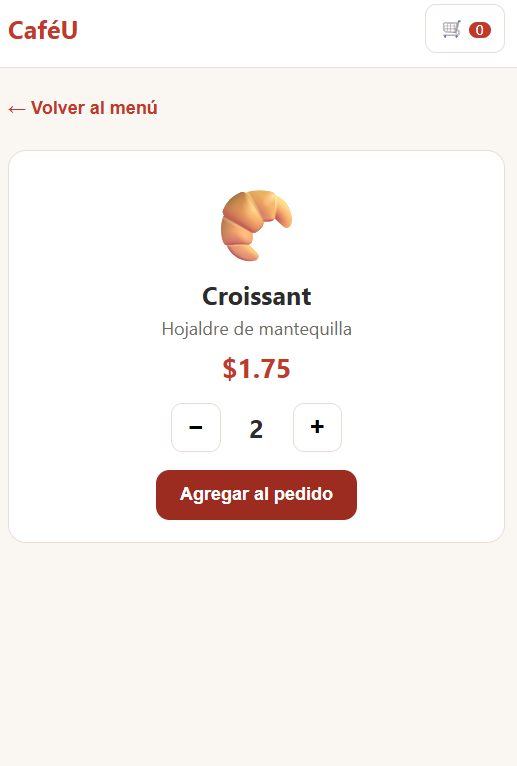
\includegraphics[width=0.48\textwidth]{imagenes/pantalla-detalle.png}
    \hfill
    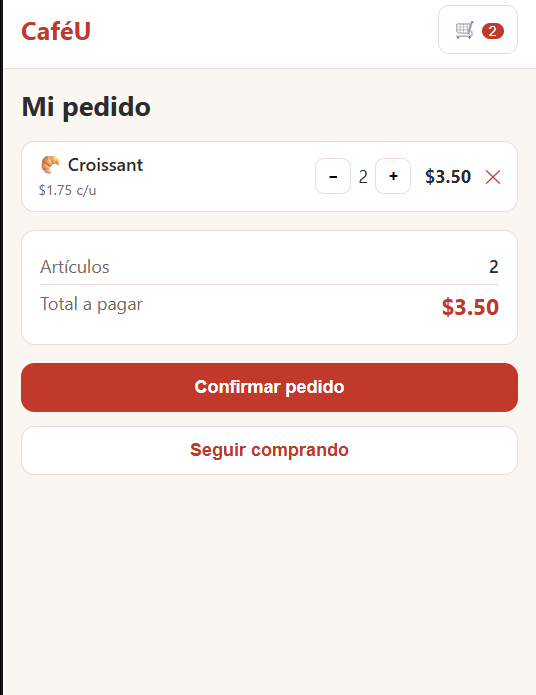
\includegraphics[width=0.48\textwidth]{imagenes/pantalla-pedido.png}
    \caption{Pantallas Detalle (selector de cantidad) y Mi pedido (desglose y subtotal).}
    \label{fig:detalle-pedido}
\end{figure}

\begin{figure}[H]
    \centering
    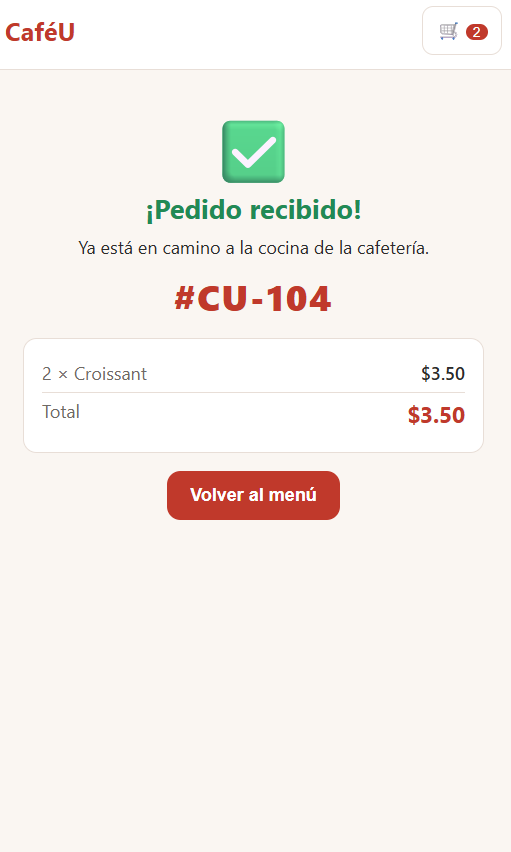
\includegraphics[width=0.5\textwidth]{imagenes/pantalla-confirmacion.png}
    \caption{Pantalla Confirmación con el código de retiro \texttt{\#CU-104}.}
    \label{fig:confirmacion}
\end{figure}

\subsubsection{Matriz de seis tareas (versión corregida)}
Las seis tareas se alinearon con el catálogo real del prototipo (café americano \$1.50, sánduche de queso \$2.75, croissant \$1.75 y tres productos de comida).

\begin{center}
\small
\begin{tabular}{|c|p{7.2cm}|p{4.5cm}|}
\hline
\textbf{ID} & \textbf{Consigna} & \textbf{Respuesta correcta} \\
\hline
T1 & ¿En qué horario atiende la cafetería? & Lunes a viernes, 7:00 a 19:00 \\
\hline
T2 & Agrega un sánduche de queso a tu pedido. & 1 sánduche (\$2,75) \\
\hline
T3 & Agrega también dos cafés americanos. & 1 sánduche y 2 cafés (\$5,75) \\
\hline
T4 & Ya no quieres el sánduche. Quítalo, confirma tu pedido y dime tu número de pedido. & \texttt{\#CU-104} (\$3,00) \\
\hline
T5 & ¿Cuántos productos de comida ofrece la cafetería? & 3 \\
\hline
T6 & ¿Cuánto pagarías por 3 croissants? & \$5,25 \\
\hline
\end{tabular}
\end{center}

\subsubsection{Ejecución del pilotaje}
Se realizaron tres sesiones individuales (unos 20 minutos cada una). En cada sesión se leyó el consentimiento informado, se verificó el perfil, se aplicó la técnica de pensamiento en voz alta y se cronometró cada tarea desde que el moderador terminaba de leer la consigna. Al finalizar, cada participante respondió el cuestionario SUS sin la mirada del moderador.

\begin{center}
\small
\begin{tabular}{|c|c|c|c|c|}
\hline
\textbf{Participante} & \textbf{Edad} & \textbf{Carrera} & \textbf{Semestre} & \textbf{Conoce el prototipo} \\
\hline
P1 & 20 & Software & 5 & No \\
\hline
P2 & 21 & Sistemas & 4 & No \\
\hline
P3 & 22 & Software & 5 & No \\
\hline
\end{tabular}
\end{center}

\subsubsection{Resultados por tarea (métricas)}
\begin{center}
\small
\begin{tabular}{|c|c|c|c|c|}
\hline
\textbf{Tarea} & \textbf{Éxito (Sí / total)} & \textbf{Mediana tiempo (s)} & \textbf{Errores críticos} & \textbf{Errores no críticos} \\
\hline
T1 · Horario & 3/3 & 6 & 0 & 0 \\
\hline
T2 · Agregar sánduche & 3/3 & 13 & 0 & 0 \\
\hline
T3 · Agregar dos cafés & 3/3 & 19 & 0 & 1 \\
\hline
T4 · Quitar y confirmar & 3/3 & 24 & 0 & 1 \\
\hline
T5 · Productos de comida & 3/3 & 8 & 0 & 0 \\
\hline
T6 · Precio de 3 croissants & 2/3 & 17 & 0 & 1 \\
\hline
\end{tabular}
\end{center}

\subsubsection{Resultados SUS (satisfacción)}
Cada participante respondió los 10 ítems del cuestionario SUS en una escala de 1 a 5. El puntaje se calcula como $(\text{impares} + \text{pares}) \times 2{,}5$, donde los ítems impares suman $(\text{valor} - 1)$ y los pares $(5 - \text{valor})$.

\begin{center}
\small
\begin{tabular}{|c|p{6.2cm}|c|c|c|}
\hline
\textbf{N°} & \textbf{Ítem SUS (resumido)} & \textbf{P1} & \textbf{P2} & \textbf{P3} \\
\hline
1 & Me gustaría usar este sistema con frecuencia & 4 & 4 & 4 \\
\hline
2 & Encontré el sistema innecesariamente complejo & 2 & 2 & 1 \\
\hline
3 & Pensé que el sistema era fácil de usar & 5 & 4 & 5 \\
\hline
4 & Necesitaría el apoyo de un técnico & 1 & 2 & 1 \\
\hline
5 & Las funciones estaban bien integradas & 4 & 4 & 4 \\
\hline
6 & Había demasiada inconsistencia & 2 & 2 & 2 \\
\hline
7 & La mayoría aprendería a usarlo rápidamente & 5 & 4 & 5 \\
\hline
8 & Encontré el sistema muy engorroso & 1 & 2 & 1 \\
\hline
9 & Me sentí muy seguro usando el sistema & 4 & 3 & 4 \\
\hline
10 & Necesité aprender muchas cosas antes & 1 & 2 & 1 \\
\hline
\multicolumn{2}{|l|}{\textbf{Puntaje SUS final ($\times$ 2,5)}} & 87,5 & 72,5 & 90,0 \\
\hline
\end{tabular}
\end{center}

\subsubsection{Ajustes del protocolo (versión 1 $\rightarrow$ versión 2)}
\begin{center}
\small
\begin{tabular}{|p{6.4cm}|p{6.4cm}|}
\hline
\textbf{Qué se observó} & \textbf{Ajuste aplicado} \\
\hline
Los precios de T2 y T4 no coincidían con el catálogo real del prototipo (sánduche \$2.25 y total \$3.50). & Se corrigieron los precios a \$2.75 (T2) y \$3.00 (T4) para que coincidan con el prototipo. \\
\hline
La consigna de T6 («¿Cuánto pagarías por 3 croissants?») resultó ambigua: un participante no supo si debía agregar los productos o solo calcular el valor. & Se reformuló la consigna como «Simula agregar 3 croissants a tu pedido y dime el total a pagar», dejando explícita la acción esperada. \\
\hline
El botón de quitar (✕) generó duda en un participante durante T4, que tardó en localizar cómo eliminar el ítem. & Se cambió el botón a «Quitar» con texto e ícono de papelera, para hacer visible la acción de eliminar. \\
\hline
\end{tabular}
\end{center}

\subsubsection{Evaluación heurística individual}
Cada integrante evaluó el prototipo de manera independiente con las 10 heurísticas de Nielsen y luego se compararon las listas, cruzándolas con los problemas observados en el pilotaje.

\begin{center}
\small
\begin{tabular}{|c|l|p{6.6cm}|}
\hline
\textbf{H} & \textbf{Heurística de Nielsen} & \textbf{Hallazgo consolidado (equipo)} \\
\hline
H1 & Visibilidad del estado del sistema & Cumple: el contador del carrito y el código \texttt{\#CU-104} informan el estado. El aviso «agregado al pedido» es breve y podría pasar desapercibido. \\
\hline
H2 & Relación entre el sistema y el mundo real & Cumple: lenguaje cotidiano del dominio de la cafetería («Agregar al pedido», «Confirmar pedido»). Sin incidencias. \\
\hline
H3 & Control y libertad del usuario & Cumple: permite quitar ítems, modificar cantidades y «Seguir comprando». Se sugiere un «Volver» más evidente desde la confirmación. \\
\hline
H4 & Consistencia y estándares & Cumple parcialmente: los botones son consistentes, pero el icono de quitar (✕) difiere del resto y generó duda en el pilotaje. \\
\hline
H5 & Prevención de errores & Cumple: el selector de cantidad limita a un mínimo de 1 y la confirmación evita el doble envío. \\
\hline
H6 & Reconocer antes que recordar & Falla (cruza con el pilotaje): el botón de quitar solo con «✕» obliga a recordar su función; un participante dudó en T4. \\
\hline
H7 & Flexibilidad y eficiencia de uso & Cumple: filtros y buscador aceleran la búsqueda. El buscador no maneja tildes (solo visible por heurística, no con usuarios). \\
\hline
H8 & Diseño estético y minimalista & Cumple: interfaz limpia, sin información irrelevante. \\
\hline
H9 & Ayudar a reconocer, diagnosticar y recuperarse de errores & Cumple parcialmente: el estado vacío del pedido orienta al usuario, pero no hay mensajes de error específicos para búsquedas sin resultados. \\
\hline
H10 & Ayuda y documentación & No aplica por tratarse de un prototipo: las tareas son autocontenidas y no requieren documentación adicional. \\
\hline
\end{tabular}
\end{center}

\subsubsection{Hallazgos preliminares (para las Fases 3 y 4)}
\begin{center}
\small
\begin{tabular}{|c|p{5.4cm}|c|c|p{2.8cm}|}
\hline
\textbf{\#} & \textbf{Problema observado} & \textbf{Tarea} & \textbf{Participantes} & \textbf{Heurística} \\
\hline
1 & El botón «✕» para quitar un ítem no es lo bastante visible y obliga a adivinar su función. & T4 & 1 de 3 & H6 \\
\hline
2 & El buscador no encuentra productos con tildes (p. ej., «sánduche» frente a «sanduche»). & Menú & 0 de 3 (solo heurística) & H7 \\
\hline
3 & El aviso «agregado al pedido» es breve y puede pasar desapercibido. & T2 / T3 & 0 de 3 (solo heurística) & H1 \\
\hline
\end{tabular}
\end{center}

\subsubsection{Evidencias de las sesiones}
Las grabaciones de pantalla y audio se mantienen en privado con autorización de los participantes. Se incluyen únicamente capturas anonimizadas de las sesiones.

\begin{figure}[H]
    \centering
    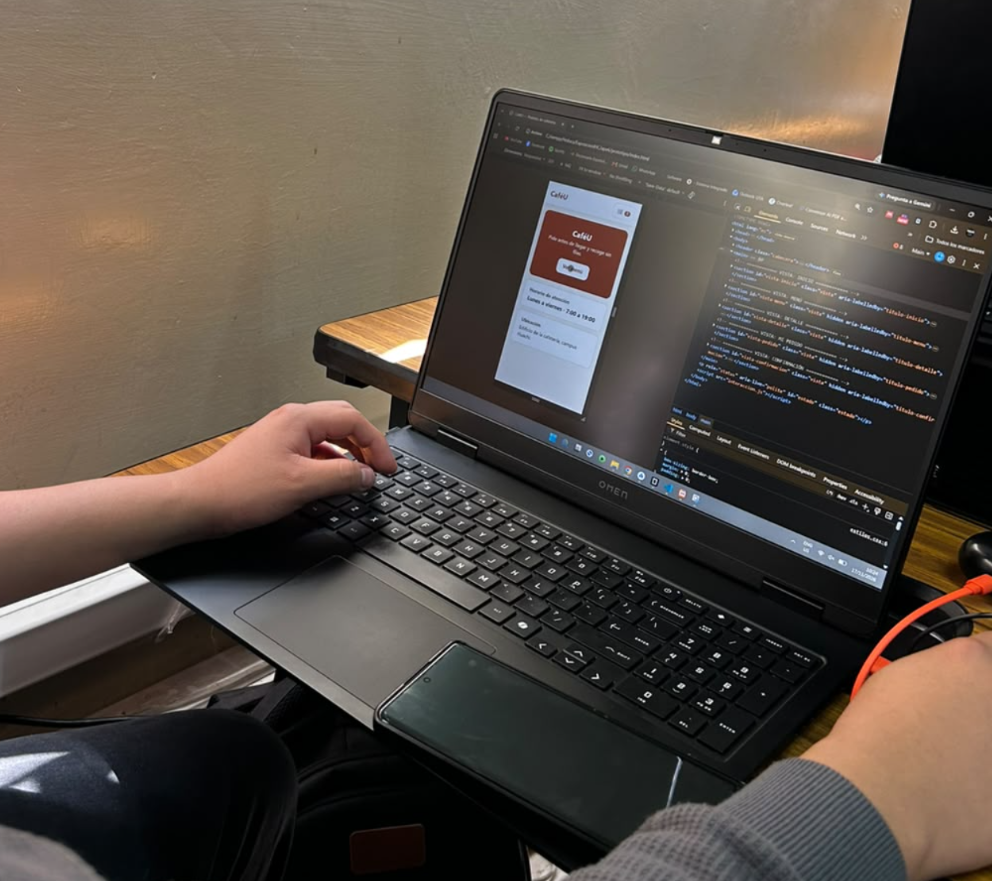
\includegraphics[width=0.3\textwidth]{imagenes/sesion-p1.png}
    \hfill
    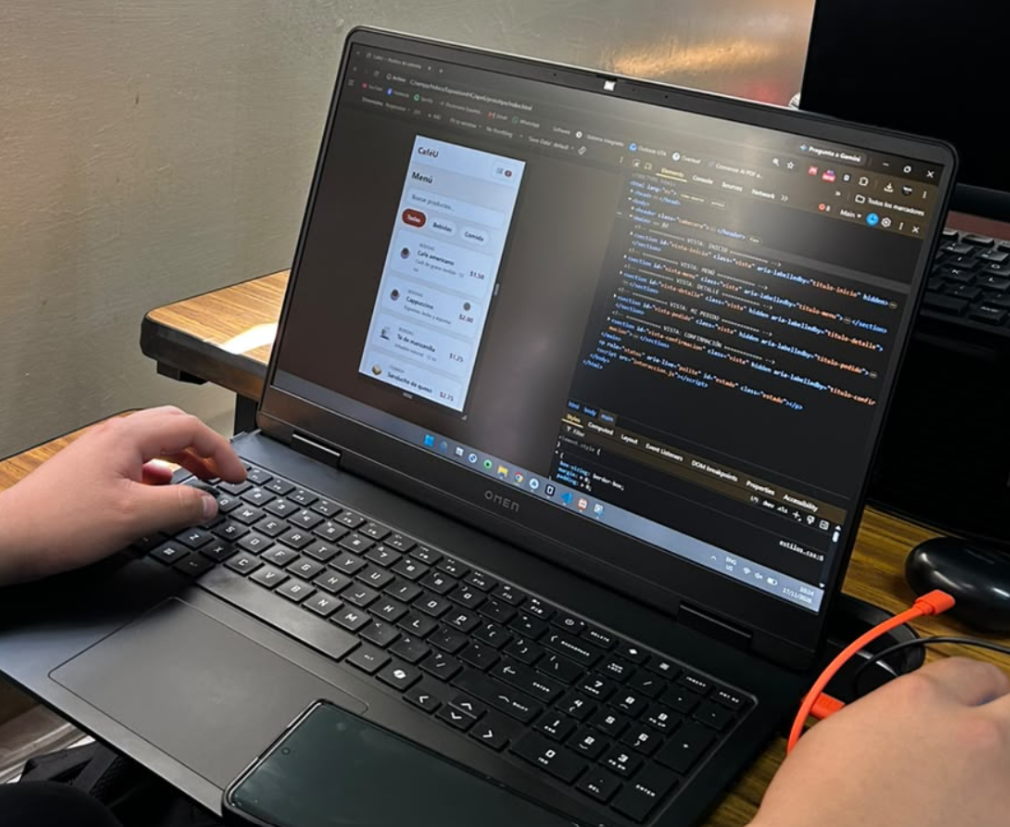
\includegraphics[width=0.3\textwidth]{imagenes/sesion-p2.png}
    \hfill
    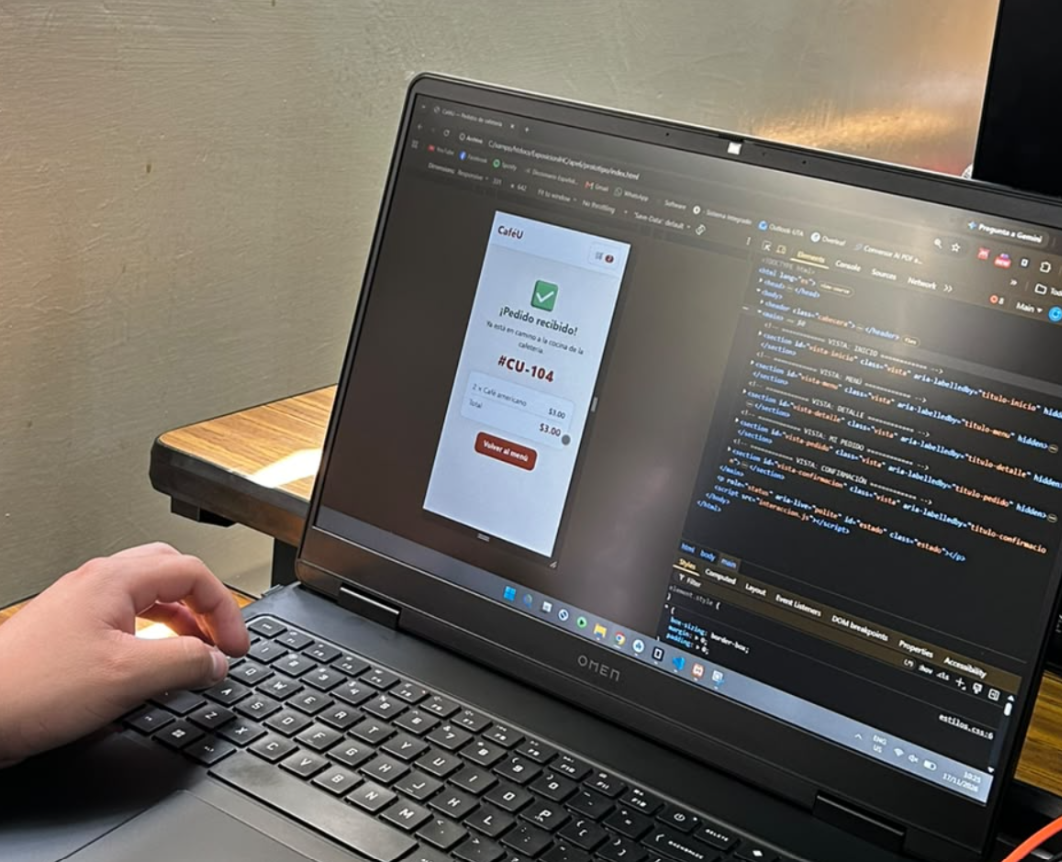
\includegraphics[width=0.3\textwidth]{imagenes/sesion-p3.png}
    \caption{Evidencia anonimizada de las sesiones con P1, P2 y P3.}
    \label{fig:sesiones}
\end{figure}

\subsubsection{Organización en GitHub}
El trabajo se mantiene en el repositorio \url{https://github.com/Sax300-cpu/HCI-2026-G2}, con la Fase 1 en \texttt{ape6/Fase1/}, el prototipo funcional en \texttt{ape6/prototipo/} y los entregables de la Fase 2 en \texttt{ape6/Fase2/}. Cada integrante evidencia su participación mediante commits identificables.

\subsection{Habilidades blandas empleadas en la práctica}
\begin{itemize}[leftmargin=1.5em, itemsep=2pt]
    \item[$\blacksquare$] Liderazgo
    \item[$\blacksquare$] Trabajo en equipo
    \item[$\blacksquare$] Comunicación asertiva
    \item[$\square$] La empatía
    \item[$\blacksquare$] Pensamiento crítico
    \item[$\square$] Flexibilidad
    \item[$\square$] La resolución de conflictos
    \item[$\square$] Adaptabilidad
    \item[$\blacksquare$] Responsabilidad
\end{itemize}

\subsection{Conclusiones}
\begin{itemize}[leftmargin=1.5em, itemsep=2pt]
    \item El pilotaje permitió comprobar si las seis tareas se entienden, si las metas de tiempo son realistas y si los instrumentos de registro sirven, antes de la evaluación completa.
    \item La tasa de éxito fue alta (17 de 18 tareas, 94 \%), con una sola tarea (T6) que requirió la pista única; las medianas de tiempo se mantuvieron dentro de las metas (6–24 s).
    \item El puntaje SUS promedio fue de 83,3 (P1 = 87,5; P2 = 72,5; P3 = 90,0), por encima del umbral de referencia de 68, lo que indica una satisfacción alta.
    \item La evaluación heurística individual cubrió aspectos que las tareas no recorren, y su cruce con el pilotaje permitió priorizar la evidencia más fuerte.
\end{itemize}

\subsection{Recomendaciones}
\begin{itemize}[leftmargin=1.5em, itemsep=2pt]
    \item Repetir la ronda con participantes del perfil si alguno no lo cumplía, para no contaminar los resultados.
    \item Mantener la pista única escrita y leída textualmente para no introducir sesgos del moderador.
    \item Designar a una sola persona para el cronómetro y registrar los tiempos en vivo (nunca estimados).
    \item Ampliar la muestra y probar con lectores de pantalla reales en iteraciones futuras.
\end{itemize}

\subsection{Referencias}
\begin{itemize}[leftmargin=1.5em, itemsep=2pt]
    \item ISO. (2018). \textit{ISO 9241-11:2018 Ergonomics of human-system interaction — Part 11: Usability: Definitions and concepts}. \href{https://www.iso.org/standard/63500.html}{iso.org/standard/63500.html}
    \item Nielsen, J. (1994). \textit{10 Usability Heuristics for User Interface Design}. Nielsen Norman Group. \href{https://www.nngroup.com/articles/ten-usability-heuristics/}{nngroup.com}
    \item Brooke, J. (1996). \textit{SUS: A quick and dirty usability scale}. In Usability Evaluation in Industry.
    \item W3C. (2023). \textit{Web Content Accessibility Guidelines (WCAG) 2.2}. \href{https://www.w3.org/TR/WCAG22/}{w3.org}
\end{itemize}

\end{document}
